%##############################################
\chapter{The standard model of particle physics}
%##############################################

\intro{An overview of the \glshere{sm} is given in the following. First, the fundamental particles and their properties are introduced. Then, the electroweak and strong interactions are detailed which includes also a brief description of the electroweak symmetry breaking mechanism. After sketching the calculation of observables in perturbation theory, the chapter is concluded by highlighting some open questions of the \gls{sm}.}

The \glshere{sm} describes the interactions between fundamental particles. It is based on \glshere{qft} which allows to predict observables of particle interactions. Exemplary observables are production cross sections or decay rates of particles which can be calculated within its framework. Validity of the \gls{sm} is constantly challenged by comparing predictions to experimental data. No significant deviations have been found so far that would hint towards physics \glshere{bsm}.


%############################################## 
\section{Particle content}
%##############################################

Fundamental particles are defined as objects for which experiments have not revealed an internal structure. For example, the upper limit on the spatial radius of the electron is measured to be $<10^{-18}~\mathrm{m}$~\cite{PhysRevLett.97.030801}. Hence, such fundamental particles are considered as point-like. They can be grouped by their spin into fermions with half-integer and bosons with integer spin. All fundamental fermions of the \gls{sm} have a spin of $\frac{1}{2}$. They can be further divided into leptons and quarks where only the latter can participate in strong interactions. Tables~\ref{tab:theory-leptons} and~\ref{tab:theory-quarks} list the leptons and quarks respectively. Each column is called a generation. It encapsulates an isospin pair whose components are therefore also referred to as up- or down-type respectively. It is unknown why there are exactly three lepton and three quark generations. Atoms which form ordinary matter consist of only particles from the first generation. These are electrons, protons, and neutrons, where the latter two are bound states of uud quarks and udd quarks respectively.

\mytable{\label{tab:theory-leptons}The leptons of the \gls{sm}. The particle masses are taken from Ref.~\cite{Olive:2016xmw}. Uncertainties on the measured masses are omitted because the precision is beyond the sub permille level. For the neutrino masses only upper \glsplfull{cl} are given.}{
    \begin{tabular}{@{}l c c c@{}}
    \toprule
                        & 1. generation                 & 2. generation                 & 3. generation \\
    \midrule
    Name                & electron neutrino             & muon neutrino                 & tau neutrino  \\
                        & ($\nu_\mathrm{e}$)            & ($\nu_{\mu}$)                 & ($\nu_{\tau}$) \\
    
    Mass                & $<225~\eV$                    & $<0.19~\MeV$                  & $<18.2~\MeV$ \\
                        & (95\% \gls{cl})                     & (90\% \gls{cl})                     & (95\%~\gls{cl})\\
    
    Electric charge     & 0                             & 0                             & 0 \\
    \midrule
    Name                & electron                      & muon                          & tau  \\
                        & ($\mathrm{e}^{\rmminus}$)     & ($\mu^{\rmminus}$)            & ($\tau^{\rmminus}$) \\
    
    Mass                & $511.0~\keV$                  & $105.66~\MeV$                 & $1.776~\GeV$ \\
                        &                               &                               &  \\
    Electric charge     & $-1$                          & $-1$                          & $-1$ \\
    \bottomrule
    \end{tabular}
}

For the masses of the neutrinos, only upper \glsplfull{cl} are known. Those are derived by combining measurements of beta decay spectra with results from neutrino oscillation experiments. When the \gls{sm} was constructed in the mid 1970s, neutrinos were assumed to be massless. However, the observation of neutrino oscillations requires that at least two neutrino generations have non-zero masses~\cite{Fukuda:1998mi}.

\mytable{\label{tab:theory-quarks}The quarks of the \gls{sm}. The u,d,s,c, and b~quark masses are reported in the \gls{msbar} mass scheme~\cite{Olive:2016xmw}. For the top quark the pole mass is quoted instead as measured in Ref.~\cite{Khachatryan:2015hba}.}{
\begin{tabular}{@{}l c c c@{}}
    \toprule
                        & 1. generation                 & 2. generation                 & 3. generation \\
    \midrule
    Name                & up (u)                        & charm (c)                     & top (t) \\
    Mass                & $2.2^{+0.6}_{-0.4}~\MeV$      & $1.27\pm0.03~\GeV$            & $172.44\pm0.49~\GeV$ \\
    
    Electric charge     & $\sfrac{2}{3}$                 & $\sfrac{2}{3}$                 & $\sfrac{2}{3}$ \\
    
    \midrule
    Name                & down (d)                      & strange (s)                   & bottom (b)  \\
    
    Mass                & $4.7^{+0.5}_{-0.4}~\MeV$      & $96^{+8}_{-4}~\MeV$           & $4.18^{+0.04}_{-0.03}~\GeV$ \\
    
    Electric charge     & $-\sfrac{1}{3}$                & $-\sfrac{1}{3}$                & $-\sfrac{1}{3}$ \\
    \bottomrule
    \end{tabular}
}


The bosons are connected to fundamental interactions by requiring invariance under a gauge group transformation as demonstrated later in this chapter. They are listed in Tab.~\ref{tab:theory-bosons}. All bosons, except the Higgs boson, carry a spin of~$1$. The Higgs boson is the only scalar fundamental particle~(spin~$0$) of the \gls{sm}. For a long time, it was a purely hypothetical particle. In July 2012, the \gls{atlas}~\cite{Aad:2012tfa} and \gls{cms}~\cite{Chatrchyan:2012xdj} collaborations independently reported the observation of a Higgs-like particle. Further investigations whether this new particle exhibits the expected interactions with other particles revealed that it is consistent with the \gls{sm} Higgs boson~\cite{Khachatryan:2016vau}. This discovery completed the \gls{sm} and thus gave further confidence into its theoretical foundation.


\mytable{\label{tab:theory-bosons}The bosons of the \gls{sm}. The Z and W~boson masses are taken from Ref.~\cite{Olive:2016xmw}. The uncertainties on their masses are omitted because the precision is beyond the sub permille level. The Higgs boson mass is taken from Ref.~\cite{Aad:2015zhl}.}{
\begin{tabular}{@{}l c c c@{}}
    \toprule
    Name     \hspace{1.6cm}           & \hspace{0.5cm}Mass\hspace{0.5cm}            & \hspace{0.5cm}Associated interaction\hspace{0.5cm}             & Gauge group \\
    \midrule
    Photon (\photon)    & $0$                  & Electromagnetism                   & $\mathrm{U(1)}$ \\
    
    Z boson   & $91.19~\GeV$         & \multirow{2}{*}{$\Bigg\}$ Weak interaction\hspace{0.3cm}}  & \multirow{2}{*}{$\mathrm{SU(2)}$}\\
    W boson   & $80.39~\GeV$         &                                    & \\
    
    Higgs boson (H)& $125.09\pm0.24~\GeV$ & Yukawa interaction                 & $\mathrm{SU(2)}\otimes\mathrm{U(1)}$\\
      
    8 gluons (g)        & $0$                  & Strong interaction                 & $\mathrm{SU(3)}$ \\  
    \bottomrule               
    \end{tabular}
}

For each fundamental particle there exists a charge-conjugated partner called antiparticle. Other properties such as mass are identical. The photon, Z boson, and Higgs boson are their own antiparticle. It is still under investigation if the neutrino is its own antiparticle. Fermions with such a property are called Majorana particles~\cite{Majorana2006}. Experimentally, this can be probed in double $\beta$ decays~($\mathrm{nn}\to\mathrm{pp}+\mathrm{e}^{\rmminus}\mathrm{e}^{\rmminus}\nu_\mathrm{e}\nu_\mathrm{e}$) where in the case of Majorana neutrinos the decay can occur without emitting two neutrinos. However, this scenario seems to be disfavored by recent results as reviewed in Ref.~\cite{Dell'Oro:2016dbc}.


%##############################################
\section{Quantum field theory}
%##############################################

In the framework of \gls{qft} particles are described as excitation modes of quantized fields. This is referred to as ``canonical'' or ``second'' quantization which allows to describe the dynamics of many-particle systems\footnote{An alternative quantization can be achieved via path integrals.}. Field operators can be decomposed as

\begin{equation}
\hat{\psi}(x)=\sum_{i}^{\mathrm{N}}u_{i}(x)\hat{a}_{i}\,,\qquad\hat{\psi}^{\dagger}(x)=\sum_{i}^{\mathrm{N}}u^{\star}_{i}(x)\hat{a}^{\dagger}_{i}\,,
\end{equation}

where $u_{i}(x)$ denotes the ordinary wave function of a single particle and $\hat{a}^{\dagger}_{i}$ ($\hat{a}_{i}$) its creation (annihilation) operator, respectively. As in classical mechanics the action of a system can be expressed as

\begin{equation}
S=\int\mathrm{L}\,\mathrm{d}t=\iint\mathcal{L}\,\mathrm{d}^{3}\vec{x}\,\mathrm{dt}=\int\mathcal{L}\,\mathrm{d}^{4}x
\end{equation}

with the Lagrangian density $\mathcal{L}$. For example, a system of free fermions is described by the Dirac Lagrangian density,

\begin{equation}
\label{eq:theory-diracL}
\mathcal{L}_\mathrm{Dirac}=\bar{\psi}\big(i\gamma^\mu\partial_\mu-m\big)\psi
\end{equation}

using the definitions $\partial_\mu\equiv\partial/\partial x_\mu$ ($\mu\in\{0\ldots3\}$) and $\bar{\psi}\equiv\psi^\dagger\gamma^{0}$, where $\gamma_\mu$ denote the Dirac matrices\footnote{Multiple representations are possible. The matrices need to satisfy a Clifford algebra with the anticommutation relation: $\big\{\gamma^\mu,\gamma^\nu\big\}=\gamma^\mu\gamma^\nu+\gamma^\nu\gamma^\mu=2g^{\mu\nu}$.}. The principle of least action, $\delta \mathrm{S}=0$, that is satisfied by the Euler-Lagrange equation yields the equation of motion as

\begin{equation}
\frac{\partial\mathcal{L}}{\partial\bar{\psi}}-\frac{\partial}{\partial_\mu}\Bigg(\frac{\partial\mathcal{L}}{\partial\big(\partial_\mu\bar{\psi}\big)}\Bigg)=\big(i\gamma^\mu\partial_\mu-m\big)\psi=0\,. \\
\end{equation}

Interactions between particles are introduced in the \gls{sm} by requiring local invariance of the Lagrangian density for certain groups of gauge transformations. This is briefly demonstrated in the following for the case of a $\mathrm{U(1)}$ transformation which leads to \glshere{qed}. Transformating Eq.~\ref{eq:theory-diracL} using 

\begin{equation}
\psi(x)\mapsto\psi^{\prime}(x)=\psi\exp^{-iq\alpha(x)}\,, \label{eq:theory-u1-trafo}
\end{equation}

yields

\begin{equation}
\mathcal{L}(\psi,\partial_\mu\psi)\mapsto\mathcal{L}(\psi^{\prime},\partial_\mu\psi^{\prime})=\bar{\psi}\,\Big(i\gamma^\mu\partial_\mu+q\,\gamma^\mu\partial_\mu\alpha(x)-m\Big)\,\psi\not=\mathcal{L}(\psi,\partial_\mu\psi)\,,
\end{equation}

where the arbitrary phase $\alpha(x)$ is a function of the local space-time coordinate $x$. The invariance $\mathcal{L}(\psi,\partial_\mu\psi)=\mathcal{L}(\psi^{\prime},\partial_\mu\psi^{\prime})$ is restored by adding a bosonic spin-1 field $\mathrm{A}_{\mu}(x)$ which interacts with $\psi$ while transforming as

\begin{equation}
\mathrm{A}_{\mu}(x)\mapsto \mathrm{A}^{\prime}_{\mu}(x)=\mathrm{A}_\mu(x)-\partial_\mu\alpha(x)\,.
\end{equation}

This procedure yields a Lagrangian density containing the following terms:

\begin{subequations}
\begin{align}
\mathcal{L}=&\hphantom{+}\bar{\psi}\,\big(i\gamma^\mu\partial_\mu-m\big)\psi &(\mathrm{fermion~propagator}) \\
            &+q\,\bar{\psi}\gamma^{\mu}\psi \mathrm{A}_{\mu} &(\mathrm{interaction}) \label{eq:theory-EM-int}\\
            &-\tfrac{1}{4}\big(\partial_\mu \mathrm{A}_\nu-\partial_\nu \mathrm{A}_\mu\big)^{2} &(\mathrm{boson~propagator})
\end{align}
\end{subequations}

In addition, the already gauge-invariant boson propagator describing the dynamics of a free $\mathrm{A}_\mu$ field has been added. The introduced interaction~(Eq.~\ref{eq:theory-EM-int}) which is required to ensure the invariance under the $\mathrm{U(1)}$ transformation~(Eq.~\ref{eq:theory-u1-trafo}) can be identified as electromagnetic interaction between a fermion described by the field $\psi$ with electric charge $q$ and a photon described by the field $\mathrm{A}_\mu$. Furthermore, the photon is predicted to be massless since adding a term of the form $m^{2}_\mathrm{A}\mathrm{A}^\mu \mathrm{A}_\mu$ would violate the invariance.

Other interactions of the \gls{sm} are also connected to local gauge transformations~(see Tab.~\ref{tab:theory-bosons}) and can thus be introduced through similar procedures. A common property follows from the Noether theorem which states that a conserved current exists for each differentiable symmetry of the action. Hence the charge associated to each gauge group is conserved. This would however be already the case for a global transformation. The invariance under an even local gauge transformations is a puzzling feature of the theory.



%##############################################
\section{Electroweak interactions and Higgs mechanism}
%##############################################
\label{sec:theory-ewk}

Electromagnetic and weak interactions can be unified using a $\mathrm{U(1)}\otimes \mathrm{SU(2)}$ gauge group. A complication arises from the fact that the $\mathrm{W}$~and $\mathrm{Z}$~bosons, mediatiors of the weak interaction, are massive. The masses of these particles have to be introduced in a different way if the concept of local gauge invariance should continue to hold. Experimentally, the UA1 and UA2 experiments at the \gls{cern} \gls{sps} proton-antiproton collider measured their masses for the first time~\cite{Arnison:1983rp,Banner:1983jy,Arnison:1983mk,Bagnaia:1983zx} while the existence of weakly-interacting charged and neutral currents was already known from bubble chamber experiments. \todo{ref? garamelle}

Another feature of weak interactions is that parity is not conserved but instead maximally violated. The interaction depends on the spin being aligned towards or against the momentum of a particle. Experimentally, the Wu experiment~\cite{PhysRev.105.1413} discovered this feature in ${}_{27}^{60}\mathrm{Co}\to{}_{28}^{60}\mathrm{Ni}+e^{\rmminus}\bar{\nu}_{e}\gamma\gamma$ decays by analyzing the direction of the escaping electron with respect to the polarization of the cobalt probe through an external magnetic field. To account for the violation of parity, fermion fields are decomposed into chiral eigenstates using the projections

\begin{align}
\psi_\mathrm{L}\equiv\mathrm{P}_\mathrm{L}\psi=\tfrac{1}{2}\big(1-\gamma_{5}\big)\psi\,,\qquad \psi_\mathrm{R}\equiv\mathrm{P}_\mathrm{R}\psi=\tfrac{1}{2}\big(1+\gamma_{5}\big)\psi
\end{align}

with $\gamma_{5}=i\gamma_{0}\gamma_{1}\gamma_{2}\gamma_{3}$\footnote{Properties: $(\gamma_{5})^{\dagger}=\gamma_{5}$; ~~$(\gamma_{5})^2=\mathrm{I}_\mathrm{4x4}$; ~~ $\{\gamma_{5},\gamma_{\mu}\}=\gamma_{5}\gamma_{\mu}+\gamma_{\mu}\gamma_{5}=0$.} where $\psi_\mathrm{L}$ ($\psi_\mathrm{R}$) is called a ``left-handed'' (``right-handed'') fermion respectively. For massless particles Eq.~\ref{eq:theory-diracL} decouples into two independent equations for $\psi_\mathrm{L}$ and $\psi_\mathrm{R}$. The chirality is then equal to the Lorentz-invariant helicity

\begin{equation}
H=\frac{\vec{p}\cdot\vec{s}}{|\vec{p}|}
\end{equation}

which denotes whether the spin $\vec{s}$ is aligned along~($H=+1$) or against~($H=-1$) the momentum. For massive particles however Eq.~\ref{eq:theory-diracL} cannot be decomposed since chirality is not Lorentz-invariant.

In the Glashow-Weinberg-Salam model~\cite{Salam:1964ry,Weinberg:1967tq,Glashow:1961tr} the fermion fields are split into left-handed doublet fields

\begin{align}
\vec{\mathrm{E}}_\mathrm{L}=\Bigg\{\colvec{2}{\nu_\mathrm{e,L}}{e^{\rmminus}_\mathrm{L}},\colvec{2}{\nu_{\mu,\mathrm{L}}}{\mu^{\rmminus}_\mathrm{L}},\colvec{2}{\nu_{\tau,\mathrm{L}}}{\tau^{\rmminus}_\mathrm{L}}\Bigg\} \label{eq:theory-su2-doublets}\,,\quad
\vec{\mathrm{Q}}_\mathrm{L}=\Bigg\{\colvec{2}{\mathrm{u}_\mathrm{L}}{\mathrm{d}_\mathrm{L}},\colvec{2}{\mathrm{c}_\mathrm{L}}{\mathrm{s}_\mathrm{L}},\colvec{2}{\mathrm{t}_\mathrm{L}}{\mathrm{b}_\mathrm{L}}\Bigg\} 
\end{align}

and right-handed singlet fields

\begin{align}
\vec{\mathrm{e}}_\mathrm{R}=\big\{\mathrm{e}^{\rmminus}_\mathrm{R},\mu^{\rmminus}_\mathrm{R},\tau^{\rmminus}_\mathrm{R}\big\},\quad\vec{\mathrm{u}}_\mathrm{R}=\big\{\mathrm{u}_\mathrm{R},\mathrm{c}_\mathrm{R},\mathrm{t}_\mathrm{R}\big\},\quad\vec{\mathrm{d}}_\mathrm{R}=\big\{\mathrm{d}_\mathrm{R},\mathrm{s}_\mathrm{R},\mathrm{b}_\mathrm{R}\big\} \label{eq:theory-su2-singlets}
\end{align}

of the $\mathrm{SU(2)}$ group. Right-handed neutrinos do not participate in any interaction within the \gls{sm}. The gauge transformation of the combined $\mathrm{U(1)}\otimes \mathrm{SU(2)}$ group is

\begin{equation}
\psi\mapsto\psi\cdot\mathrm{e}^{-ig\vec{\alpha}(x)\cdot\vec{\omega}/2}\cdot\mathrm{e}^{-ig^{\prime}\beta(x)/2} \label{eq:theory-u1su2-transformation}
\end{equation}

where $\omega_{a}$~($a\in\{1,2,3\}$) denote the Pauli matrices and $g$, $g^{\prime}$ the corresponding conserved charges. This leads to four boson fields, $\mathrm{W}^{a}$ and $\mathrm{B}$, that interact with the fermions. In analogy to Eq.~\ref{eq:theory-EM-int} one obtains

\begin{align}
\mathcal{L}_\mathrm{interaction}=~~\sum_{\psi_\mathrm{L}}^\mathrm{doublets}&\bar{\psi}^{i}_\mathrm{L}~\gamma^{\mu}\Big(\tfrac{1}{2}g\vec{\mathrm{W}}_{\mu}\cdot\vec{\omega}+\tfrac{1}{2}g^{\prime}\mathrm{B}_{\mu}\Big)\psi^{i}_\mathrm{L} \nonumber\\
+\sum_{\psi^{i}_\mathrm{R}}^\mathrm{singlets}&\bar{\psi}^{i}_\mathrm{R}~\gamma^{\mu}\tfrac{1}{2}g^{\prime}\mathrm{B}_{\mu}\psi^{i}_\mathrm{R} + \mathrm{\gls{hc}} \label{eq:theory-codev-su2-interaction}
\end{align}

where the summation is implied over the fermion doublet and singlet components.

A fermion mass term $ m_\mathrm{f}\bar{\psi}{}_\mathrm{f}\psi_\mathrm{f}=m_\mathrm{f}(\bar{\psi}{}_\mathrm{f,L}\psi_\mathrm{f,R}+\bar{\psi}_\mathrm{f,R}\psi_\mathrm{f,L})$ cannot be added to the Lagrangian density since it is not invariant under $\mathrm{SU(2)}$ transformation. This is solved by Englert-Brout-Higgs-Guralnik-Hagen-Kibble-mechanism~\cite{HIGGS1964132,PhysRevLett.13.508,PhysRevLett.13.321,PhysRevLett.13.585} which introduces mass terms not only for fermions but also for the gauge bosons through symmetry breaking. For this, a new scalar $\mathrm{SU(2)}$ doublet field $\phi=(\phi^{\rmplus},\phi^{0})$\footnote{$\phi^{\rmplus}$ annihilates positively charge scalar particles / creates antiparticles with negative charge; $\phi^{0}$ annihilates neutral particles / creates neutral antiparticles.}, invariant under $\mathrm{U(1)}\otimes\mathrm{SU(2)}$ transformation, is added to the Lagrangian density

\begin{subequations}
\begin{align}
\mathcal{L}_{\phi}&=\big(D_{\mu}\phi^{\dagger}\big)\big(D^{\mu}\phi\big)+\mathrm{V}(\phi) \label{eq:theory-phi-propagator} \\
D^{\mu}\phi&=\big(\partial^{\mu}+\tfrac{1}{2}ig\vec{\mathrm{W}}^{\mu}\cdot\vec{\omega}+\tfrac{1}{2}ig^{\prime}\mathrm{B}^{\mu}\big)\phi \label{eq:theory-phi-codev}
\end{align}
\end{subequations}

which interacts with the gauge bosons. In addition, $\phi$ has a potential 

\begin{equation}
\mathrm{V}(\phi)=-\mu^2\phi^\dagger\phi+\tfrac{1}{2}\lambda(\phi^\dagger\phi)^2
\end{equation}

in the form of a ``Mexican hat'' as shown in Fig.~\ref{fig:theory-higgs-potential} that leads to a non-zero \glshere{vev} for $\mu^2>0$ of 

\begin{equation}
\phi_0=\sqrt{\frac{\mu^{2}}{2\lambda}}\equiv \frac{v}{\sqrt{2}}\,.
\end{equation}

\myfigure{\label{fig:theory-higgs-potential}The ``Mexican hat'' potential of the Higgs field with a non-zero \glshere{vev} $\phi_0$ which leads to symmetry breaking.}{
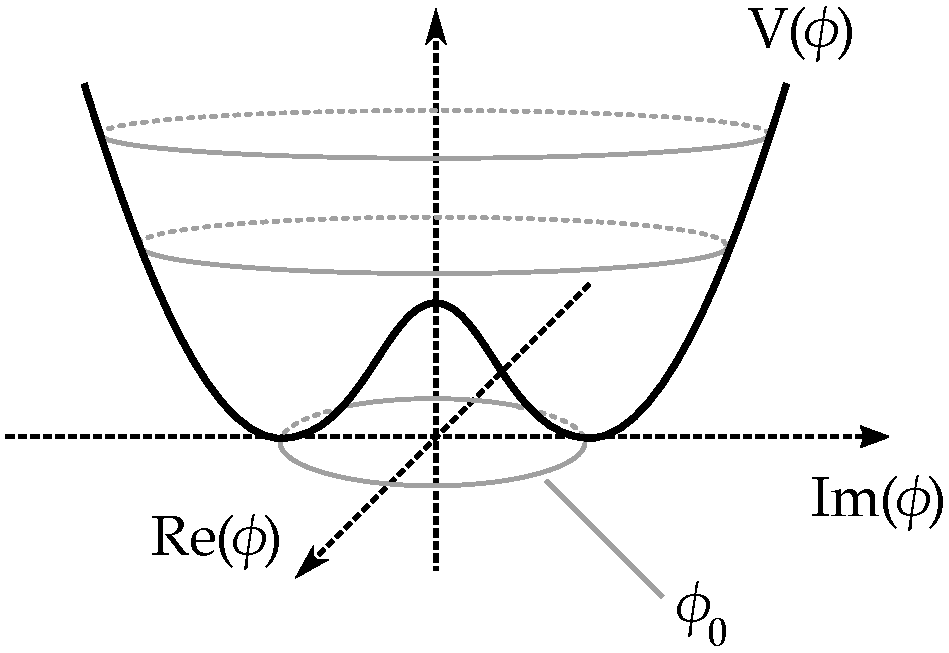
\includegraphics[width=0.5\textwidth]{figures/theory/higgspot.pdf}
}

One says that this shifted \gls{vev} ``breaks'' the $\mathrm{SU(2)}$ symmetry when parameterizing $\phi$ around the minimum of $V(\phi)$ as

\begin{equation}
\phi(x) \Bigg|_{\phi_0} =~\frac{1}{\sqrt{2}}\colvec{2}{0}{v+\mathrm{H}(x)}\cdot \exp\left(-i\,\frac{\vec{\theta}(x)\cdot\vec{\omega}}{2v}\right)\,, \label{eq:theory-phi-dev}
\end{equation}

where $\vec{\theta}$ denotes three so-called ``Goldstone'' bosons and $\mathrm{H}$ the Higgs boson. In fact, the symmetry still exists but is ``hidden''. A $\mathrm{SU(2)}$ transformation called ``unitary gauge'' can be performed such that $\vec{\theta}$ vanishes. One says that these three Goldstone bosons and their degrees of freedom are ``eaten'' by the $\mathrm{W}$ and $\mathrm{Z}$~bosons to become massive. Hence, through the extra degree of freedom they can also have a longitudinal polarization after symmetry breaking. The parametrization is chosen such that it leaves the minimum invariant under the $\mathrm{U(1)}$ subgroup transformation

\begin{equation}
\phi\mapsto\phi\cdot\mathrm{e}^{-ig\alpha_{3}(x)\omega_{3}/2}\cdot\mathrm{e}^{-ig^{\prime}\beta(x)/2}. \label{eq:theory-broken-u1-trans}
\end{equation}

Inserting Eq.~\ref{eq:theory-phi-dev} into Eq.~\ref{eq:theory-phi-propagator} yields amongst others the following Lagrangian densities capturing the non-interacting terms:

\begin{subequations}
\begin{align}
\mathcal{L}_\mathrm{Higgs}=&\hphantom{-}\tfrac{1}{2}(\partial_{\mu}\mathrm{H}^{\dagger})(\partial^{\mu}\mathrm{H})-\lambda^2 v^2 \mathrm{H}^2 \label{eq:theory-higgs} \\
\mathcal{L}_\mathrm{W_1,W_2~bosons}=&-\tfrac{1}{4}\big(\mathrm{W}_{1,\mu\nu}\mathrm{W}^{\mu\nu}_{1}+\mathrm{W}_{2,\mu\nu}\mathrm{W}^{\mu\nu}_{2}\big)\nonumber\\&+\tfrac{1}{8}g^2 v^2 \big(\mathrm{W}_{1,\mu} \mathrm{W}_{1}^{\mu}+\mathrm{W}_{2,\mu} \mathrm{W}_{2}^{\mu}\big) \label{eq:theory-a1a2} \\
\mathcal{L}_\mathrm{W_3,B~bosons}=&-\tfrac{1}{4}\big(\mathrm{B}_{\mu\nu}\mathrm{B}^{\mu\nu}+\mathrm{W}_{3,\mu\nu}\mathrm{W}^{\mu\nu}_{3}\big)\nonumber\\
&+\tfrac{1}{8}v^2 \big(g\mathrm{W}_{3,\mu}-g^{\prime}\mathrm{B}_\mu\big)\big(g\mathrm{W}_{3}^{\mu}-g^{\prime}\mathrm{B}^\mu\big) \label{eq:theory-a3b}.
\end{align}
\end{subequations}

The first term (Eq.~\ref{eq:theory-higgs}) describes the free scalar Higgs boson with mass $m_\mathrm{H}=\lambda v$. Next, the $\mathrm{W}_{1}$ and $\mathrm{W}_{2}$
fields in Eq.~\ref{eq:theory-a1a2} can be identified as a particle/antiparticle pair $\mathrm{W}^{\pm}=(\mathrm{W}_1\mp i\mathrm{W}_2)/\sqrt{2}$ with mass $m_\mathrm{W}=\frac{1}{2}gv$. Lastly, the fields $\mathrm{W}_3$ and $\mathrm{B}$ appear to be in a mixed mass state in Eq.~\ref{eq:theory-a3b}. By performing a rotation of the couplings

\begin{equation}
\colvec{2}{\mathrm{Z}}{\mathrm{A}}=\begin{pmatrix}
\cos\theta_\mathrm{W} & -\sin\theta_\mathrm{W} \\
\sin\theta_\mathrm{W} & \cos\theta_\mathrm{W}
\end{pmatrix}
\colvec{2}{\mathrm{W}_{3}}{\mathrm{B}}\,,\qquad \cos\theta_\mathrm{W}=\frac{g}{\sqrt{g^2+g^{\prime 2}}}\,,
\end{equation}

where $\theta_\mathrm{W}$ is called the ``weak-mixing'' or ``Weinberg'' angle, another massive boson, the $\mathrm{Z}$~boson, with mass $m_\mathrm{Z}=v\sqrt{g^2+g^{\prime2}}/2$ and a massless boson $\mathrm{A}_\mu$, the photon, can be identified. The angle is determined as $\sin^2\theta_\mathrm{W} \approx 0.23$~\cite{Olive:2016xmw} through the couplings $g$ and $g^\prime$. Equation~\ref{eq:theory-phi-propagator} also yields the relation $\rho=m_\mathrm{W}^{2}/(m_\mathrm{Z}^{2}\cdot\cos\theta_\mathrm{W}^{2})=1$ which is called ``custodial symmetry''. Rewriting the covariant derivative of Eq.~\ref{eq:theory-phi-codev} into these mass eigenstates yields

\begin{align}
D_\mu=&\hphantom{-}\partial_\mu~+~i\frac{g}{\sqrt{2}}\cdot\Big(\mathrm{W}^{\rmplus}_\mu T^{\rmplus}+\mathrm{W}^{\rmminus}_\mu T^{\rmminus}\Big)\nonumber\\
&-i\,\frac{g^2\,T_3-g^{\prime 2}\,Y}{\sqrt{g^2+g^{\prime 2}}}\cdot\mathrm{Z}_\mu~-~i\,\frac{g^{\prime}g\,\big(T_3+Y\big)}{\sqrt{g^2+g^{\prime 2}}}\cdot \mathrm{A}_\mu \label{eq:theory-codev-breaking}
\end{align}

where $T^{\pm}$ denote the ladder operators, $Y$ the $\mathrm{U(1)}$ so-called ``hyper'' charge, and $T_3$ the $\mathrm{SU(2)}$ charge. From the coupling to the photon one can read off the electric coupling constant to be 

\begin{equation}
e=\frac{g^{\prime}\,g}{\sqrt{g^2+g^{\prime 2}}}
\end{equation}

which is measured as $\aem=e^2/(4\pi)\approx1/137$~\cite{Olive:2016xmw} and the corresponding electric charge to be $Q=T_3+Y$ which is invariant under Eq.~\ref{eq:theory-broken-u1-trans}. For the weak coupling constant one finds the relation $e=g\cdot\sin\theta_\mathrm{W}$ which yields $\aw=\aem/\sin^2\theta_\mathrm{W}\approx0.032$. The value of the \gls{vev} can be estimated from muon lifetime measurements through the Fermi coupling constant as $v=(\sqrt{2}\,\mathrm{G}_\mathrm{F})^{-1/2}\approx 246~\GeV$~\cite{PhysRevLett.106.041803}. A consequence of electroweak symmetry breaking is the prediction of the Higgs boson which was finally discovered in July 2012 independently by the \gls{atlas}~\cite{Aad:2012tfa} and \gls{cms}~\cite{Chatrchyan:2012xdj} collaborations and thus completed the electroweak theory.


Fermion masses can be generated as well by interacting with the Higgs field. One introduces Yukawa interactions as

\begin{subequations}
\begin{align}
\mathcal{L}_\mathrm{Yukawa~lepton~int.}=&-\lambda_{e}^{ii}\cdot\bar{\mathrm{E}}^{i}_\mathrm{L}\phi\cdot\mathrm{e}^{i}_\mathrm{R}+\mathrm{\gls{hc}} \label{eq:theory-lepton-yukawa}\\
\mathcal{L}_\mathrm{Yukawa~quark~int.}=&-\lambda_{d}^{ij}\cdot\bar{\mathrm{Q}}^{i}_\mathrm{L}\phi\cdot\mathrm{d}^{j}_\mathrm{R}-\lambda_{u}^{ik}\cdot\bar{\mathrm{Q}}^{i}_\mathrm{L}\epsilon^{ij}\phi\cdot\mathrm{u}^{k}_\mathrm{R} +\mathrm{\gls{hc}} \label{eq:theory-quark-yukawa}
\end{align}
\end{subequations}

where the coupling strengths are denoted by $\lambda$. After the symmetry breaking a mass term for the electron, muon and tau lepton of $m_\ell=-\lambda_\ell v/\sqrt{2}$ is introduced. The quarks can be disentangled from their mixed mass state through a rotation of the fields 

\begin{equation}
\mathrm{u}^{i}_\mathrm{L}\mapsto U^{ij}_\mathrm{u}\mathrm{u}^{j}_\mathrm{L},\qquad \mathrm{d}^{i}_\mathrm{L}\mapsto U^{ij}_\mathrm{d}\mathrm{d}^{j}_\mathrm{L}
\end{equation}

which allows to write the Lagrangian density in the quark mass eigenstates. In particular, using Eqs.~\ref{eq:theory-codev-su2-interaction} and~\ref{eq:theory-codev-breaking} this yields the interactions

\begin{subequations}
\begin{align}
\mathcal{L}_{\mathrm{W}\bar{\mathrm{f}}\mathrm{f}~\mathrm{int.}}=\hphantom{+}i&\frac{g}{2\sqrt{2}}\,\Big[\bar{\nu}_{i}(\gamma^\mu-\gamma^\mu\gamma^5) \mathrm{W}^{\rmplus}_\mu\,\ell^{\rmminus}_{i}~+~{\ell}^{\rmplus}_{i}(\gamma^\mu-\gamma^\mu\gamma^5) \mathrm{W}^{\rmminus}_\mu\,\nu_{i}\Big]\nonumber\\
+i&\frac{g}{2\sqrt{2}}\,\Big[\mathrm{V}_{ij}\,\bar{\mathrm{u}}_{i}(\gamma^\mu-\gamma^\mu\gamma^5) \mathrm{W}^{\rmplus}_\mu\,\mathrm{d}_{j}~+~\mathrm{V}_{ij}^\dagger\,\bar{\mathrm{d}}_{i}(\gamma^\mu-\gamma^\mu\gamma^5) \mathrm{W}^{\rmminus}_\mu\,\mathrm{u}_{j}\Big] \label{eq:theory-qqW-int}
\end{align}
\end{subequations}

between the $\mathrm{W}$~bosons and fermions where $\mathrm{V}_{ij}=(U^\dagger_\mathrm{u}U_\mathrm{d})_{ij}$ denotes the \glshere{ckm} matrix. Its elements are free parameters of the \gls{sm} and have to be measured experimentally. A global fit using a multitude of measurements~\cite{Olive:2016xmw} while assuming unitarity for the three quark generations yields

\begin{equation}
\begin{pmatrix}
\ckm{ud} & \ckm{us} & \ckm{ub} \\
\ckm{cd} & \ckm{cs} & \ckm{cb} \\
\ckm{td} & \ckm{ts} & \ckm{tb} 
\end{pmatrix}
~=~
\begin{pmatrix}
0.974 & 0.225 & 0.004 \\
0.225 & 0.974 & 0.041 \\
0.009 & 0.040 & 0.999 
\end{pmatrix}\,.
\end{equation}

The coupling structure, $\gamma_{\mu}-\gamma_{\mu}\gamma_{5}$, between $\mathrm{W}$~bosons and the fermions is referred to as a \glshere{va} structure because of its spatial transformation properties. Axial vectors do not switch sign under parity transformation  unlike normal spatial vectors\footnote{A typical example of an axial vector (also known as pseudovector) is the angular momentum $\vec{L}=\vec{r}\times \vec{p}$.}. This allows only left-handed fermions or right-handed antifermions to couple to $\mathrm{W}$~bosons as observed by the Wu experiment.



%##############################################
\section{Strong interactions}
%##############################################
\label{sec:theory-qcd}

The theory of \glshere{qcd} describes the strong interaction between quarks and gluons. It is connected to a $\mathrm{SU(3)}$ gauge group resulting into the Lagrangian density of

\begin{align}
\mathcal{L}_\mathrm{\gls{qcd}}=\bar{\psi}i\gamma^{\mu}\big(\partial_{\mu}-ig\vec{\mathrm{G}}_\mu\vec{\lambda}\big)\psi-\tfrac{1}{4}\vec{\mathrm{G}}_{\mu\nu}\vec{\mathrm{G}}^{\mu\nu},\qquad \psi=\colvec{3}{\psi_\mathrm{red}}{\psi_\mathrm{green}}{\psi_\mathrm{blue}}
\end{align}

which is invariant under the transformation

\begin{equation}
\psi\mapsto\psi\mathrm{e}^{-ig\vec{\alpha}(x)\vec{\lambda}}\,.
\end{equation}

The fields $\vec{\mathrm{G}}_\mu$ describe eight gluons which represent the massless gauge bosons of the group. The conserved charge of the group is called ``color'' (red, green, blue) which is however equal in strength for all charges. The generators $\lambda_a$~($a\in{1\ldots8}$) obey the relation $[\lambda_a,\lambda_b]=if_{abc}\lambda^c$ with the antisymmetric structure constant $f_{abc}$. A common representation of $\vec{\lambda}$ is given by the Gell-Mann matrices. The non-abelian group structure leads to gluon self-interactions through the gluon field strength tensor

\begin{equation}
\mathrm{G}_{\mu\nu}^{a}=\partial_{\mu} \mathrm{G}_\nu^{a}-\partial_{\nu} \mathrm{G}_{\mu}^{a}+gf^{abc}\mathrm{G}_{\mu,b}\mathrm{G}_{\nu,c}\,.
\end{equation}

No free quarks can exist in nature because of a phenomenon called ``color-confinement''. The \gls{qcd} potential between two quarks can be approximated as a ``Coulomb-plus-linear'' potential~\cite{Sumino2003173}

\begin{equation}
V(r)=-\frac{4\cdot\as}{3r}+k\cdot r\,,
\end{equation}

where a linear term dominates at large distances $r$ or equivalently small exchanged energies. The factor $k$ can be understood as a ``gluon-spring'' tension similar to that of a harmonic oscillator. New quark/antiquark pairs can be created from the vacuum if the gluon field energy exceeds the mass of the new pair. This can lead to a cascade of particles emerging from the gluon field at sufficiently large energies which bind ``free'' quarks into color-neutral singlets called hadrons. Such a process is referred to as hadronization. In experiments, one usually clusters therefore collimated particles into a jet whose momentum is then used to infer the momentum of a quark or gluon candidate at its origin.

Hadrons can be either mesons which consist of quark-antiquark pairs~($\bar{\mathrm{q}}\mathrm{q}$) or baryons consisting of quark triplets~($\mathrm{qqq}$). These constituents of a hadron are referred to as ``valence quarks''. Common mesons are the pions $\uppi^{\rmplus}$~($\mathrm{u}\bar{\mathrm{d}}$), $\uppi^{0}$~($(\mathrm{u}\bar{\mathrm{u}}-\mathrm{d}\bar{\mathrm{d}})/\sqrt{2}$), kaons $\mathrm{K}^{\rmplus}$~($\mathrm{u}\bar{\mathrm{s}}$), $\mathrm{K}^{0}$~($\mathrm{d}\bar{\mathrm{s}}$) and $\mathrm{J}/\Psi$~($\mathrm{c}\bar{\mathrm{c}}$). Typical baryons are the proton~($\mathrm{uud}$), the neutron~($\mathrm{udd}$), and~$\Lambda^{0}$~($\mathrm{uds}$). The baryon number, $\mathrm{B}\equiv N\text{(baryons)}-N\text{(antibaryons)}$, is conserved in interactions. In 2003, a new bound state containing four quarks has been observed by the Belle experiment~\cite{PhysRevLett.91.262001} at \gls{kek}, Japan. The \gls{lhcb} experiment at the \gls{lhc}, \gls{cern} confirmed this observation in 2013~\cite{Aaij:2013zoa} followed by the discovery of more so-called ``tetraquark'' candidates~\cite{Aaij:2014jqa,Aaij:2016iza} and even ``pentaquarks'' forming a bound state of five quarks~\cite{Aaij:2015tga}.

Besides valence quarks and gluons, virtual quarks, so-called ``sea quarks'', are considered constituents of a hadron as well. This whole group of particles is commonly referred to as partons. In hadron collision experiments at a sufficiently high momentum transfer, one can approximate all partons as free which allows to treat hadron-hadron scattering as a single parton-parton interaction instead~\cite{Feynman:1969wa}. The momentum of a parton is expressed as a fraction of the hadron momentum $\vec{p}_\mathrm{parton}=x\cdot \vec{p}_\mathrm{hadron}$. Then, the probability of 
finding two parton flavors $f_{i}$ with momentum fraction $x_{i}$ interacting at an energy scale $\mu_\mathrm{F}$ in a hadron-hadron collision is given by the \glshere{pdf} as $\mathrm{\gls{pdf}}(x_{1},f_{1},\mu_\mathrm{F})\cdot\mathrm{\gls{pdf}}(x_{2},f_{2},\mu_\mathrm{F})$. The \glspl{pdf} are normalized such that

\begin{equation}
\sum_{f}^\mathrm{partons}\int_{0}^{1}\mathrm{d}x~x\cdot \mathrm{PDF}(x,\mu_\mathrm{F},f)=1
\end{equation}

yields the total momentum of the hadron. The scale $\mu_\mathrm{F}$ is called ``factorization scale'' below which non-perturbative low energy effects such as soft gluon emissions have been absorbed into the \gls{pdf}. Measuring the \glspl{pdf} at scale $\mu_\mathrm{F}$, one can extrapolate them to any other scale by solving the DGLAP\footnote{Named after the authors: Y. Dokshitzer, W. Gribow, L. Lipatow, G. Altarelli, G. Parisi} equation~\cite{Dokshitzer:1977sg,Gribov:1972ri,Altarelli:1977zs}. A review of common \gls{pdf} sets which are currently used in descriptions of \gls{lhc} collisions can be found in Ref.~\cite{Accardi2016}. There are various groups estimating \gls{pdf} sets from fits to experimental data using different approaches; e.g. CTEQ, MMHT~(formerly MSTW), ABM, HERAPDF, and NNPDF. Exemplary distributions taken from the NNPDF group~(version 3.0), using the \LHAPDF[format=hyperbf] library~\cite{Buckley:2014ana}, are shown in Fig.~\ref{fig:theory-nnpdf-dist} for $\mu_\mathrm{F}=10~\GeV$ and $\mu_\mathrm{F}=100~\GeV$. More information on this \gls{pdf} set can be found in Ref.~\cite{Ball:2014uwa}. At a momentum fraction of $x\approx0.2$ one can observe an excess of the up and down quark distributions as expected from the valence quark composition of the proton. These vanish at low momentum fractions at which the contributions from sea quarks and the gluon dominate.

\myfigure{\label{fig:theory-nnpdf-dist}NNPDF\,$3.0$ \gls{nnlo} PDF set in 5 flavor scheme for $\as(m_\mathrm{Z})=0.118$ and factorization scales of (a)~$10~\GeV$ and (b)~$100~\GeV$. The gluon \gls{pdf} has been scaled down by a factor of $0.1$.}{
\subfloat[]{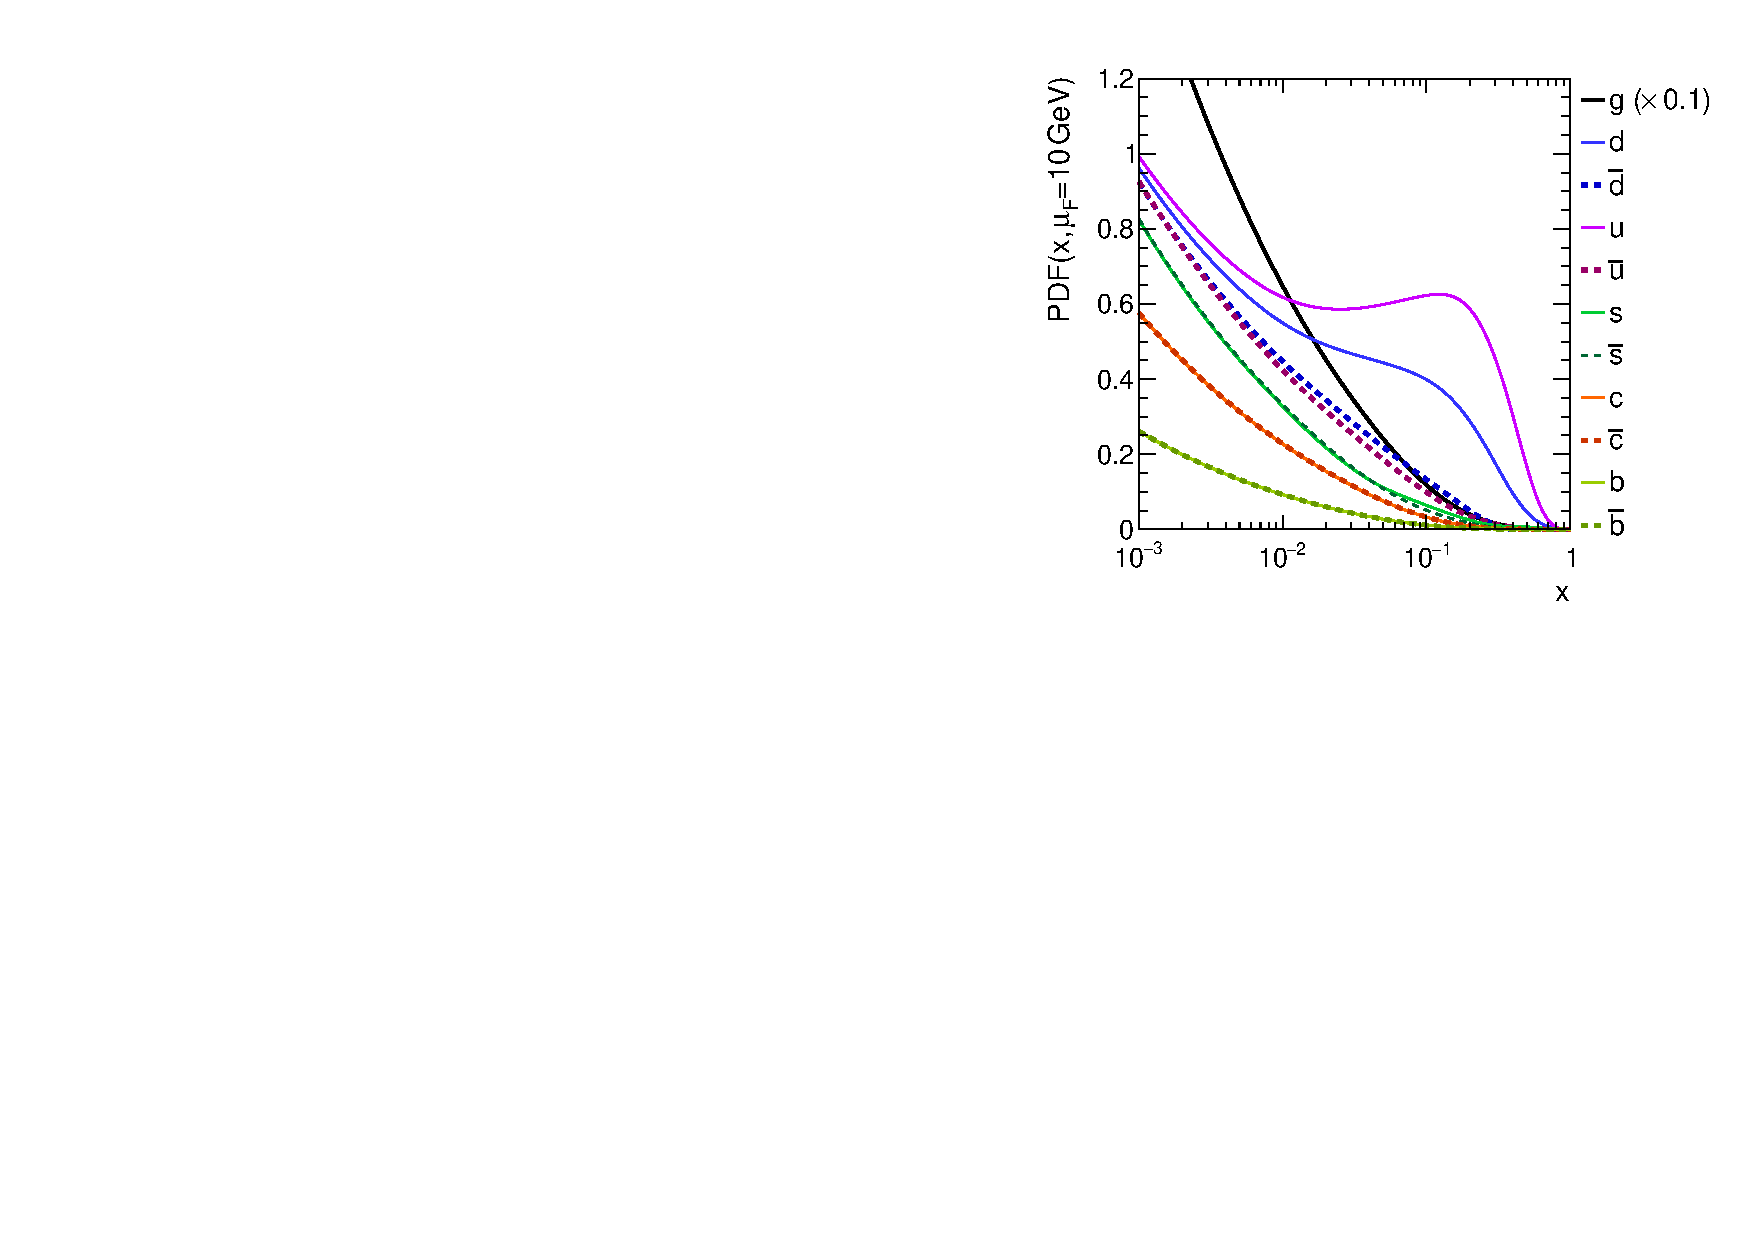
\includegraphics[width=0.49\textwidth]{figures/theory/nnpdf_q10.pdf}}\hspace{0.01\textwidth}
\subfloat[]{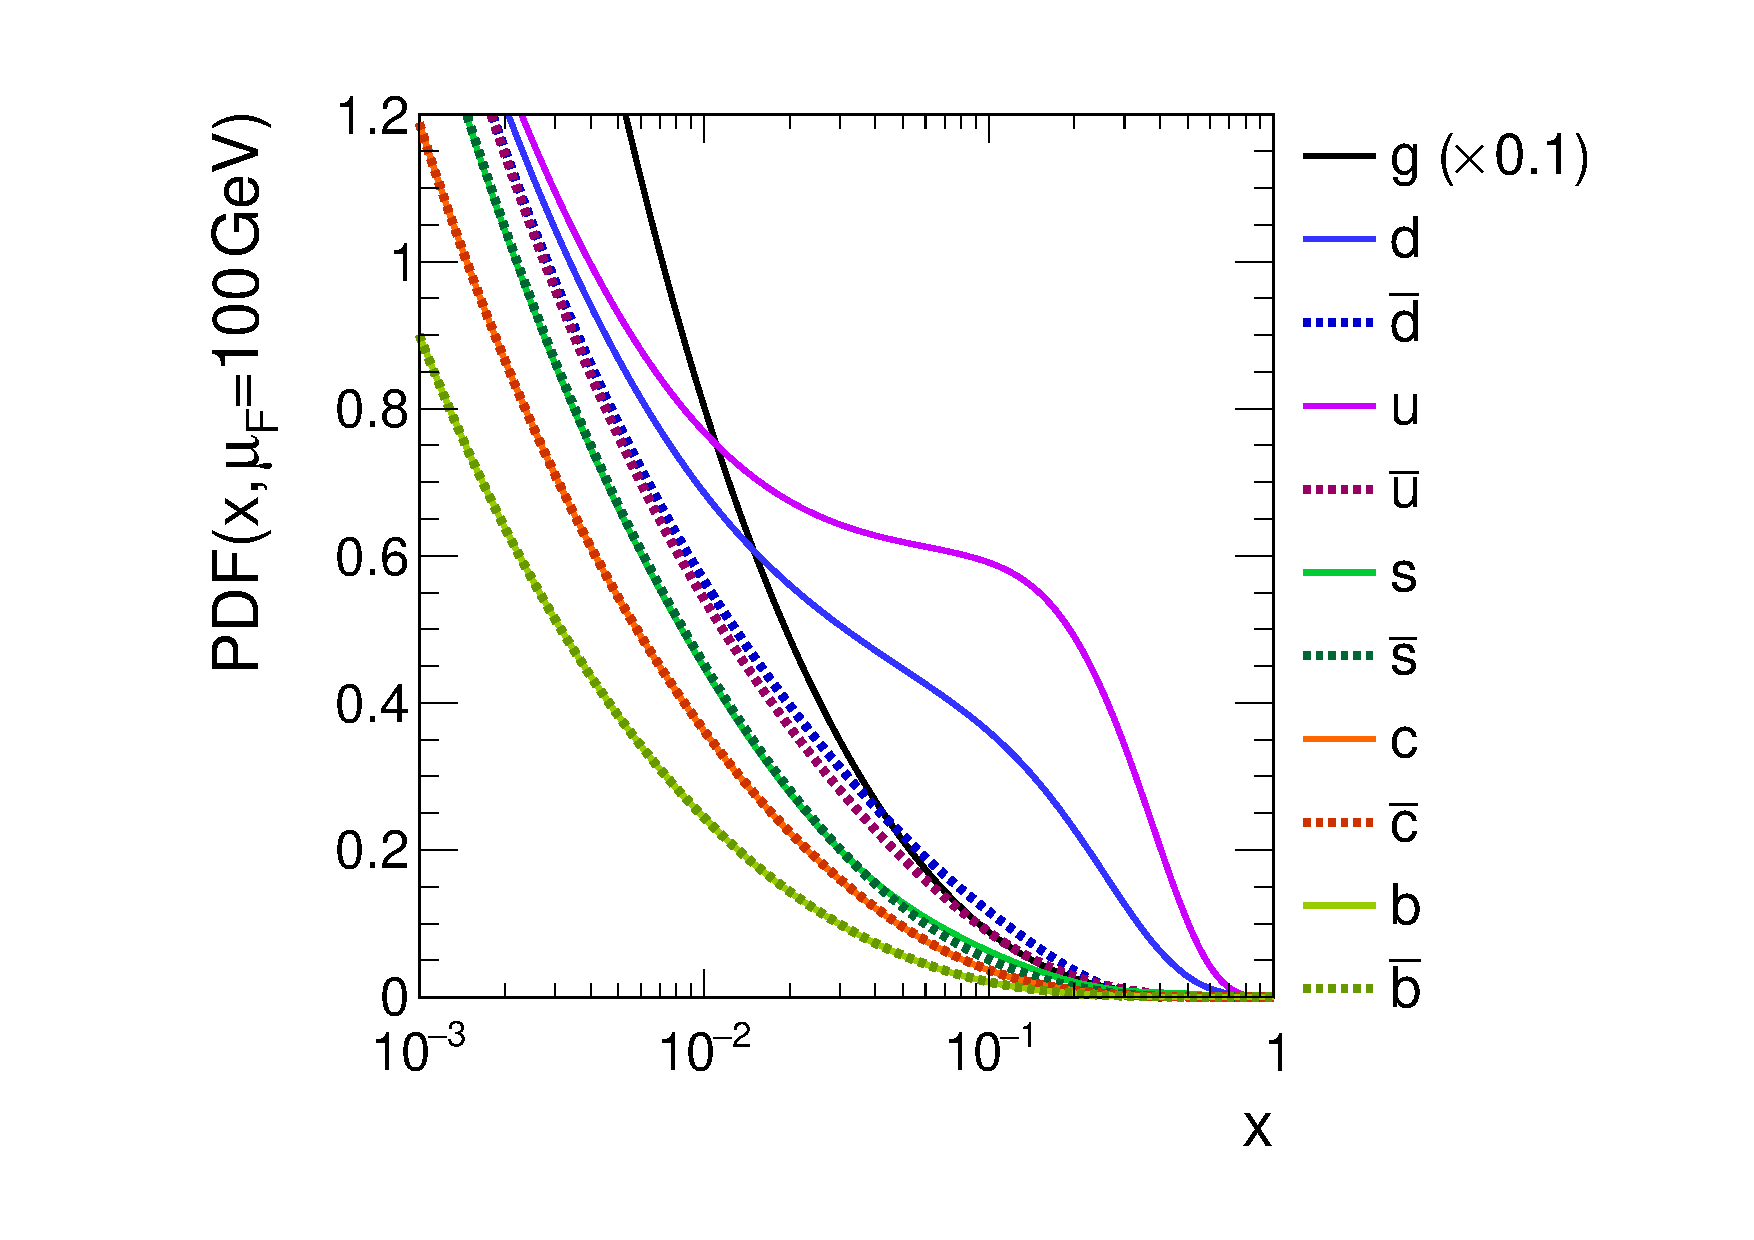
\includegraphics[width=0.49\textwidth]{figures/theory/nnpdf_q100.pdf}}
}

At high energies, quantum fluctuations lead to divergences. In order to let a theory still describe the experimental energy regime, physical quantities are redefined at the so-called ``renormalization scale'' $\mu_\mathrm{R}$. This leads amongst others to a ``running'' behavior of the coupling constants as a function of $\mu_\mathrm{R}$. Beyond this scale, high energy effects such as loop corrections to propagators~(``self-energy'') are absorbed in the physical quantities through a renormalization of the fields. In particular, the running behavior of the strong coupling constant is found to be 

\begin{equation}
\as(\mu_\mathrm{R})=\frac{\as(\mu_{0}^{2})}{1+\as(\mu_\mathrm{0}^2)\cdot\tfrac{33-2\cdot n_f}{12\pi}\cdot\ln\Big(\tfrac{|\mu_\mathrm{R}^2|}{\mu_{0}^{2}}\Big)}
\end{equation}

where $n_f$ denotes the number of quarks and $\mu_{0}$ is a reference scale where the coupling is known from measurements, e.g. $\mu_{0}=m_\mathrm{Z}$. The world average of the strong coupling constant $\as=g/(4\pi^2)$ at the $\mathrm{Z}$~boson mass is currently estimated to be $\as(m_\mathrm{Z})=0.1181\pm0.0011$~\cite{Olive:2016xmw}. 

Quarks can be treated as ``asymptotically free'' since the strong coupling decreases towards larger energies. On the other hand, following the behavior of $\as(\mu^2_\mathrm{R})$ to lower energies, a limit $\Lambda_\mathrm{\gls{qcd}}\approx 200~\MeV$ is found at which $\as$ becomes even larger than one. Below such energies, perturbative calculations of observables can no longer be performed~(see Sec.~\ref{sec:theory-observables}). 





%##############################################
\section{Observables}
%##############################################
\label{sec:theory-observables}

A particle scattering process or decay is fully characterized by the initial and final state particles as well as the interactions between them. Experimental observables are inclusive and differential cross sections as well as decay rates which can be calculated using perturbation theory. The cornerstone of such a calculation is the \glshere{smatrix} which describes the transition probability of a system from an initial to a final multiparticle state as $|\langle i|\mathcal{S}|f\rangle|^{2}$. In the Heisenberg picture the \gls{smatrix} is given by the Dyson series

\begin{align}
\mathcal{S}&=\mathrm{T}\Big[\exp\Big(-i\int\mathrm{d}^{4}x~\mathcal{H}_\mathrm{int}(t)\Big)\Big]\\
&=\sum_{n=0}^{\infty}\frac{(-i)^{n}}{n!}\int_{-\infty}^{\infty}\mathrm{d}^{4}x_{1}\ldots \int_{-\infty}^{\infty}\mathrm{d}^{4}x_{n}~\mathrm{T}\Big[\mathcal{H}_\mathrm{int}(t_{1})\ldots\mathcal{H}_\mathrm{int}(t_{n})\Big] \label{eq:theory-dyson-series}
\end{align}

where particle interactions are described within the non-free part of the Hamiltonian density $\mathcal{H}_\mathrm{int}=\mathcal{H}-\mathcal{H}_\mathrm{free}$. The operator $\mathrm{T}$ ensures that products of $\mathcal{H}_\mathrm{int}(t_{i})$ are ordered by time. Typically one captures the interaction terms for $n\geq1$ of Eq.~\ref{eq:theory-dyson-series} into a \glshere{me} denoted $\mathcal{M}$ instead. If $\mathcal{H}_\mathrm{int}>1$ the series does not converges and one says the problem is not solvable perturbatively. For instance, the ground states of hadrons can not be calculated perturbatively because of the running of the strong coupling constant. An alternative approach based on lattice gauge theory allowed to solve this problem~\cite{Durr:2008zz}.

For a scattering process, given a flux $L=\rho v$ of incoming particles with density $\rho$ and velocity $v$, the cross section $\sigma$ is defined as the number of interactions per unit density~($\rho=1$). It is usually denoted in the unit ``barn''~[$\mathrm{b}$] which is defined as $1~\mathrm{b}\equiv 10^{-28}~\mathrm{m}^{2}$.  The number of interaction events per time is given by $\mathrm{d}N/\mathrm{d}t=L\sigma$. The flux $L$ is commonly referred to as luminosity. In the case of hadron-hadron collisions the total cross section can be calculated from the partonic cross section $\sigma(f_{i}f_{j}\to X)$ for a given process  as

\begin{equation}
\sigma(\mathrm{pp}\to X)=\sum_{i,j}\iint\mathrm{d}x_{1}\,\mathrm{d}x_{2}~\mathrm{PDF}(x_{1},f_{i})\,\mathrm{PDF}(x_{2},f_{j})\,\sigma(f_{i}f_{j}\to X)\,,
\end{equation}

where additional summations and integrations over the \glspl{pdf} are required to account for the individual contributions per incoming parton flavor $f_{i}$ and momentum fraction $x_{i}$.

Cross sections can be written in terms of the number of interaction vertices contributing to $\mathcal{M}$ originating from the perturbative series~(Eq.~\ref{eq:theory-dyson-series}). This allows to the expand them as a power series in terms of the coupling constant $\alpha$ as

\begin{equation}
\sigma=\sigma_\mathrm{\gls{lo}}\Big(1+\frac{\alpha}{2\pi}\cdot\sigma_\mathrm{1}+\big(\frac{\alpha}{2\pi}\big)^2\cdot\sigma_{2}+\big(\frac{\alpha}{2\pi}\big)^{3}\cdot\sigma_{3}+\ldots\Big).
\end{equation}

Depending at which term the series is cut off one speaks of \glshere{lo}, \glshere{nlo}, or \glshere{nnlo} accuracy in $\alpha$. In general, it is desirable to calculated observables beyond \gls{lo}. Predictions including higher order corrections tend to be less affected by theoretical uncertainties which originate from a variation of the chosen renormalization and factorization scales\footnote{Partonic \gls{lo} cross sections can only be monotonous functions of $\mu_\mathrm{R}$ since $\sigma\propto\alpha(\mu_\mathrm{R})$. Hence, an uncertainty due to a scale variation can be even considered meaningless.}.

The optical theorem, which can be derived from the unitarity $\mathcal{S}^{\dagger}\mathcal{S}=1$ of the \gls{smatrix}, states that the imaginary part of a forward scattering amplitude $\mathcal{M}(i\to f)$ is directly related to the total scattering amplitude of producing all possible intermediate particles $\sum_{X}\mathcal{M}^\dagger(i/f\to X)$ from the inital or final state. Since a total cross section is at least as big as the single forward scattering cross section one finds that the matrix elements are bound and cannot be arbitrary large. Nonetheless, a theory may describe experimental data well but violates the unitarity bound at higher energies. Such a case would hint towards a new physics model which restores unitarity by introducing new particles or interactions above the experimentally probable energy regime. This is called \glshere{uv} completion. Hence, a unitarity-violating theory may just reflect the low energy limit of an unknown \gls{uv}-complete theory. Exemplary, the $\mathrm{W}^{\rmplus}\mathrm{W}^{\rmminus}\to\mathrm{W}^{\rmplus}\mathrm{W}^{\rmminus}$ scattering amplitude would grow as $\mathcal{M}\sim s/m_\mathrm{W}^2$ if there is no Higgs boson and eventually violate unitarity at $\sqrt{s}\approx1~\TeV$.


%##############################################
\section{Open questions}
%##############################################

The \gls{sm} is believed to be not the final theory describing fundamental interactions. In the following, some of its problems are briefly outlined.

\begin{description}
\item[Gravity] The \gls{sm} cannot describe gravitational interactions. Its mediator, the graviton, would have to be a spin~2 boson which however leads non-renormalizable divergences. However, at energy scales reached by colliders, it is fine to ignore gravitational interactions since those become only comparable in strength to the electroweak and strong interactions at the Planck scale which is $\mathcal{O}(10^{18}~\GeV)$ if there are no extra dimensions.
\item[Naturalness] A large correction to the bare Higgs boson mass originates from top quark loops due to Yukawa interactions. Those need to be absorbed by the physical mass through renormalization. The resulting mass can be written as $m^{2}_\mathrm{H}\approx m_\mathrm{bare}+\lambda_\mathrm{t}^{2}\mu^2/(16\pi^2)$. If the \gls{sm} is valid up to the Planck scale it would require an extraordinary fine-tuning of the bare Higgs mass in order to cancel this large correction. Such a coincidence is considered to be not very ``natural''.
\item[Dark matter and dark energy] Cosmological observations of rotation speeds of galaxies, mapping of matter distributions through micro-lensing, and acoustic oscillations in the cosmic microwave background suggest that there exists a yet unidentified kind of matter, called ``dark matter''. An even more puzzling building block of the universe which is missing from the \gls{sm} is dark energy. It is a crucial ingredient to describe the expansion of the universe.

\end{description}

